\documentclass[11pt,a4paper]{article}
\usepackage[T1]{fontenc}
\usepackage[utf8]{inputenc}
\usepackage[french]{babel}
\usepackage{lmodern}
\usepackage{microtype}
\usepackage[margin=2.4cm]{geometry}
\usepackage{amsmath,amssymb,amsthm,mathtools,bm}
\usepackage{booktabs,tabularx,array}
\usepackage{graphicx}
\usepackage{xcolor}
\usepackage{enumitem}
\usepackage{caption}
\usepackage[hidelinks]{hyperref}
\usepackage{tikz}
\usetikzlibrary{arrows.meta,positioning,calc}

\definecolor{accent}{HTML}{2A78D6}
\definecolor{edgec}{HTML}{EB6834}
\definecolor{cloudc}{HTML}{1BAF7A}
\definecolor{muted}{HTML}{5A6270}
\hypersetup{colorlinks=true,linkcolor=accent,urlcolor=accent,citecolor=accent}
\graphicspath{{../results/figures/}}

\newtheorem{definition}{Définition}
\newcommand{\E}{\mathbb{E}}
\newcommand{\R}{\mathbb{R}}
\newcommand{\ind}{\mathbf{1}}
\setlist{itemsep=2pt,topsep=4pt}
\captionsetup{font=small,labelfont=bf}

\title{\textbf{MARL-Offload}\\[4pt]
\large Apprentissage par renforcement multi-agent pour le délestage de calcul\\
dans un système edge--cloud, avec tarification leader--suiveurs}
\author{Ossama Sabti}
\date{Novembre 2026}

\begin{document}
\maketitle

\begin{abstract}
\noindent Six appareils hétérogènes reçoivent des tâches de calcul et décident, tâche par tâche, de les exécuter
localement, sur un serveur \emph{edge} partagé ou dans le \emph{cloud}. Le serveur edge est une ressource
congestionnable : les décisions des uns ralentissent les autres. Nous formalisons ce problème comme un jeu de
Markov partiellement observable à somme générale, puis nous comparons trois algorithmes d'apprentissage
multi-agent (IQL, IPPO, MAPPO) à des règles de décision simples. Nous étudions ensuite une variante hiérarchique
où l'opérateur du serveur fixe un prix d'accès, et nous mesurons la distance des politiques obtenues à un
équilibre de Nash. Les apprenants réduisent le coût par tâche de 10 à 12\,\% par rapport à une règle myope, et
leurs politiques sont proches d'un équilibre. Une règle myope munie d'un péage de congestion bien réglé atteint
le même coût moyen, mais elle n'est pas stable : chaque appareil aurait intérêt à ne pas la respecter.
\end{abstract}

\tableofcontents
\newpage

%======================================================================
\section{Contexte et question}
%======================================================================

Les téléphones, caméras, capteurs ou véhicules connectés doivent exécuter des calculs de plus en plus lourds
(vision, reconnaissance vocale, inférence de réseaux de neurones). Trois options s'offrent à chaque appareil :
\begin{itemize}
  \item \textbf{calculer localement}, ce qui est lent pour un petit processeur et coûteux en énergie ;
  \item \textbf{délester vers un serveur edge}, un serveur de proximité rapide mais \emph{partagé} ;
  \item \textbf{délester vers le cloud}, sans congestion mais avec un aller-retour long et des frais.
\end{itemize}
Le problème du \emph{délestage de calcul} (\emph{computation offloading}) consiste à choisir, pour chaque tâche,
l'option qui minimise un compromis entre latence, énergie et coût monétaire.

La difficulté vient du partage. Si tous les appareils envoient leurs tâches au serveur edge au même moment, une
file d'attente se forme et tout le monde attend. Chaque appareil ne connaît que sa propre situation et une
indication \emph{retardée} de la charge du serveur ; il ne voit pas ce que décident les autres. Le projet pose
deux questions :
\begin{enumerate}
  \item des apprenants indépendants, qui n'utilisent que de l'information locale, peuvent-ils se coordonner
        mieux qu'une règle myope ?
  \item si l'opérateur du serveur fixe un prix d'accès en anticipant la réaction des appareils, quel prix
        choisit-il, et ce prix est-il bon pour l'ensemble du système ?
\end{enumerate}

\begin{figure}[h]
\centering
\begin{tikzpicture}[font=\small, >=Stealth,
  dev/.style={draw=accent, rounded corners=3pt, minimum width=2.3cm, minimum height=0.55cm, fill=accent!8},
  srv/.style={draw=#1, rounded corners=4pt, line width=1pt, minimum width=3.1cm, minimum height=1.1cm, fill=#1!8, align=center}]
  \foreach \i/\f in {1/0{,}6,2/0{,}7,3/0{,}8,4/0{,}9,5/1{,}0,6/1{,}2} {
    \node[dev] (d\i) at (0,{-0.75*\i}) {appareil \i \; ($f_\i=\f$)};
  }
  \node[srv=edgec] (edge) at (6.4,-1.9) {\textbf{Edge}\\ $F=3$ unités/pas\\ file FIFO partagée};
  \node[srv=cloudc] (cloud) at (6.4,-4.2) {\textbf{Cloud}\\ délai $D=1{,}5$, frais $\varphi=0{,}3$};
  \foreach \i in {1,...,6} {
    \draw[->, edgec!80, thin] (d\i.east) -- (edge.west);
    \draw[->, cloudc!70, thin, dashed] (d\i.east) -- (cloud.west);
  }
  \draw[->, muted, dashed, thick] (edge.north) to[bend right=40] node[above, text=muted]{signal de charge retardé ($d=2$)} (d1.north);
\end{tikzpicture}
\caption{Le système étudié : six appareils de vitesses différentes, un serveur edge partagé et un cloud.}
\label{fig:systeme}
\end{figure}

%======================================================================
\section{Modèle mathématique}
%======================================================================

\subsection{Agents, temps et tâches}

On considère $N=6$ agents $i\in\{1,\dots,N\}$ et un horizon fini de $H=50$ pas de temps $t=0,\dots,H-1$.
À chaque pas, l'agent $i$ reçoit une tâche avec probabilité $p=0{,}8$ :
\[
  z_{i,t}\sim\mathrm{Bernoulli}(p),\qquad
  w_{i,t}\sim\mathcal{U}[0{,}5;\,1{,}5]\ \text{(taille, en unités de travail)} .
\]
Le flux moyen de travail est donc $N\,p\,\E[w]=6\times0{,}8\times1=4{,}8$ unités par pas, alors que le serveur
edge en traite $F=3$ : il ne peut pas absorber toutes les tâches, et les appareils doivent se le partager.

Chaque agent possède une vitesse de calcul locale $f_i\in\{0{,}6;0{,}7;0{,}8;0{,}9;1{,}0;1{,}2\}$ et un canal
radio $c_{i,t}\in\{0,1\}$ (mauvais ou bon) qui suit une chaîne de Markov à deux états :
\[
  \Pr(c_{i,t+1}=c_{i,t})=\rho_i,\qquad \rho=(0{,}9;\,0{,}95;\,0{,}8;\,0{,}85;\,0{,}9;\,0{,}7).
\]
Le débit montant vaut $R(1)=2$ et $R(0)=0{,}5$. Envoyer une tâche prend un temps
$\tau_{i,t}=\delta\,w_{i,t}/R(c_{i,t})$, avec $\delta=0{,}5$ unité de données par unité de travail.

\subsection{Actions et coûts}

Chaque agent qui a une tâche choisit une action $a_{i,t}\in\{0,1,2\}$ = \{local, edge, cloud\}. Son coût est
\begin{equation}
  C_{i,t} = L_{i,t} + \lambda\,E_{i,t} + P_{i,t},
  \qquad r_{i,t}=-C_{i,t},
\end{equation}
où $L$ est la latence, $E$ l'énergie (poids $\lambda=1$) et $P$ le paiement. Un agent sans tâche a un coût nul.

\paragraph{Local ($a=0$).} La tâche attend derrière la file locale $q_{i,t}$ de l'appareil :
\[
  L = \frac{q_{i,t}+w_{i,t}}{f_i},\qquad E=\kappa\,f_i^2\,w_{i,t}\ (\kappa=0{,}5),\qquad P=0,
\]
et la file locale évolue selon $q_{i,t+1}=\max\bigl(0,\;q_{i,t}+w_{i,t}\ind[a_{i,t}=0]-f_i\bigr)$.
Le terme en $f_i^2$ traduit le fait qu'un processeur rapide consomme plus d'énergie.

\paragraph{Edge ($a=1$).} Soit $\mathcal{E}_t$ l'ensemble des agents qui choisissent l'edge au pas $t$, servis
dans un ordre aléatoire $\sigma$, et $B_t$ la file résiduelle du serveur. Le $k$-ième agent servi attend tout
le travail placé devant lui, y compris le sien :
\[
  L_{\sigma(k)} = \tau_{\sigma(k)} + \frac{B_t+\sum_{j\le k} w_{\sigma(j)}}{F},
  \qquad E=p_{\mathrm{tx}}\,\tau,\qquad P=\pi ,
\]
où $p_{\mathrm{tx}}=0{,}3$ est la puissance d'émission et $\pi$ le prix fixé par l'opérateur ($\pi=0$ hors
variante hiérarchique). La file du serveur persiste d'un pas à l'autre :
\begin{equation}
  B_{t+1}=\max\Bigl(0,\;B_t+\sum_{i\in\mathcal{E}_t} w_{i,t}-F\Bigr).
  \label{eq:file}
\end{equation}
C'est cette dynamique qui couple les agents : une décision d'aujourd'hui augmente la latence de tous demain.

\paragraph{Cloud ($a=2$).} Pas de congestion, mais un aller-retour fixe et des frais :
\[
  L=\tau+D+\frac{w}{F_c},\qquad E=p_{\mathrm{tx}}\,\tau,\qquad P=\varphi,
  \qquad D=1{,}5,\ F_c=10,\ \varphi=0{,}3 .
\]

\subsection{Observations : une information partielle et retardée}

L'agent $i$ n'observe pas l'état complet. Son observation $o_{i,t}\in\R^9$ contient :
\[
  o_{i,t}=\Bigl(z_{i,t},\ \tfrac{w_{i,t}}{1{,}5},\ \min\!\bigl(\tfrac{q_{i,t}}{5},2\bigr),\ c_{i,t},\ f_i,\
  \min\!\bigl(\tfrac{B_{t-d}}{10},2\bigr),\ \tilde\pi,\ \tfrac{t}{H},\ \tfrac{i-1}{N-1}\Bigr),
\]
soit sa tâche, sa file locale, son canal, sa vitesse, un signal public de la charge du serveur \textbf{vieux de
$d=2$ pas}, le prix normalisé $\tilde\pi$, le temps et son indice. Il ne voit ni la charge actuelle $B_t$, ni les
files et canaux des autres, ni leurs décisions simultanées.

L'\emph{état global} $s_t$, utilisé seulement par le critique centralisé de MAPPO, concatène les observations de
tous les agents et la vraie charge actuelle $B_t/10$.

\subsection{Le jeu}

\begin{definition}[Jeu de Markov partiellement observable à somme générale]
Le système est un tuple $\bigl(N,\mathcal{S},\{\mathcal{A}_i\},\{\mathcal{O}_i\},T,\{r_i\},H,\gamma\bigr)$
où la transition $T(s_{t+1}\mid s_t,\bm a_t)$ est décrite ci-dessus et chaque agent reçoit sa propre récompense
$r_i$. Une politique (décentralisée) de l'agent $i$ est $\pi_i(a\mid o_i)$, et son objectif est
\begin{equation}
  J_i(\pi_i,\pi_{-i}) = \E_{\pi}\Bigl[\sum_{t=0}^{H-1}\gamma^t\,r_{i,t}\Bigr].
\end{equation}
\end{definition}

Le jeu est à \emph{somme générale} : chaque appareil minimise son propre coût, pas le coût total.

\begin{definition}[Équilibre de Nash]
Un profil de politiques $\pi^\star$ est un équilibre de Nash si aucun agent ne peut améliorer son objectif en
changeant seul de politique :
$\ J_i(\pi_i^\star,\pi_{-i}^\star)\ \ge\ J_i(\pi_i,\pi_{-i}^\star)$ pour tout $i$ et tout $\pi_i$.
\end{definition}

\paragraph{Coût social.} Le prix $\pi$ payé à l'opérateur est un \emph{transfert} entre acteurs du système, pas
une perte. Le coût social par tâche compte donc la latence, l'énergie et les frais cloud (payés à l'extérieur),
mais pas le prix edge :
\begin{equation}
  \mathrm{SC} = \frac{\sum_{i,t}\bigl(L_{i,t}+\lambda E_{i,t}+\varphi\,\ind[a_{i,t}=2]\bigr)}{\sum_{i,t} z_{i,t}} .
\end{equation}

%======================================================================
\section{Politiques de référence}
%======================================================================

\paragraph{Règles triviales.} Tout local, tout edge, tout cloud, et le choix uniforme au hasard.

\paragraph{Règle myope (\emph{greedy}).} Chaque agent estime le coût des trois options à partir de son
observation, en prenant le signal retardé $\hat B=B_{t-d}$ comme charge actuelle et en supposant que personne
d'autre n'utilise l'edge au même pas :
\[
  \hat C_{\text{edge}} = \tau + \frac{\hat B + w}{F} + \lambda p_{\mathrm{tx}}\tau + \pi,\quad
  \hat C_{\text{local}} = \frac{q+w}{f_i}+\lambda\kappa f_i^2 w,\quad
  \hat C_{\text{cloud}} = \tau + D + \frac{w}{F_c} + \lambda p_{\mathrm{tx}}\tau + \varphi ,
\]
puis choisit $\arg\min$. C'est une meilleure réponse myope : elle ignore à la fois l'effet de ses propres décisions
sur le futur et les décisions simultanées des autres.

\paragraph{Règle myope avec péage (\emph{greedy+toll}).} Même règle, avec un surcoût virtuel $\theta$ ajouté à
$\hat C_{\text{edge}}$. Ce péage n'est payé à personne ; il fait \emph{internaliser} à chaque appareil une partie
de la congestion qu'il impose aux autres, à la manière d'un péage pigouvien. Le paramètre est choisi par
recherche sur grille $\theta\in\{0;0{,}1;\dots;1{,}2\}$ sur des épisodes de réglage distincts des épisodes
d'évaluation. La valeur retenue est $\theta=0{,}8$.

%======================================================================
\section{Méthodes d'apprentissage}
%======================================================================

\subsection{Rappels d'apprentissage par renforcement}

Pour un seul agent, la fonction de valeur d'action d'une politique $\pi$ est
$Q^\pi(o,a)=\E_\pi\bigl[\sum_{k\ge0}\gamma^k r_{t+k}\mid o_t=o,a_t=a\bigr]$, et la fonction optimale vérifie
l'équation de Bellman
\begin{equation}
  Q^\star(o,a)=\E\bigl[r+\gamma\max_{a'}Q^\star(o',a')\bigr].
\end{equation}
Dans un système multi-agent, les autres agents font partie de l'environnement de chacun. Comme ils apprennent en
même temps, l'environnement vu par un agent est \emph{non stationnaire} : c'est la difficulté centrale de
l'apprentissage multi-agent.

Les trois méthodes utilisent le \textbf{partage de paramètres} : un seul réseau sert à tous les agents.
L'indice de l'agent et sa vitesse $f_i$ font partie de l'observation, de sorte que la politique peut quand même
différer d'un appareil à l'autre. Les réseaux sont des perceptrons à deux couches cachées de 64 neurones
(activation $\tanh$). Les récompenses sont multipliées par $1/3$ pour stabiliser l'apprentissage.

\subsection{IQL : Q-learning profond indépendant}

Chaque agent apprend $Q_\theta(o_i,a)$ comme s'il était seul. Les transitions $(o,a,r,o',\mathrm{fin})$ de tous
les agents sont stockées dans une mémoire de rejeu de $10^5$ éléments. La cible utilise le \emph{double DQN},
qui découple le choix de l'action (réseau courant $\theta$) de son évaluation (réseau cible $\bar\theta$, recopié
tous les 500 pas) pour réduire la surestimation :
\begin{equation}
  y = r + \gamma\,(1-\mathrm{fin})\,Q_{\bar\theta}\bigl(o',\arg\max_{a'}Q_\theta(o',a')\bigr).
\end{equation}
La perte est la perte de Huber $\ell_\delta\bigl(Q_\theta(o,a)-y\bigr)$, minimisée par Adam (pas $5\cdot10^{-4}$,
lots de 256). L'exploration est $\varepsilon$-gloutonne, avec $\varepsilon$ qui décroît linéairement de 1 à
0{,}05 sur les 60\,\% premiers épisodes.

Les transitions où l'agent n'a pas de tâche sont conservées (récompense nulle). Les ignorer laisserait $Q_\theta$
non entraîné sur ces observations, alors qu'elles apparaissent comme états suivants $o'$ dans la cible.

\subsection{PPO : optimisation de politique par gradient}

PPO apprend directement une politique stochastique $\pi_\phi(a\mid o)$ et un critique $V_\psi$. À partir de
trajectoires collectées avec l'ancienne politique $\pi_{\phi_{\text{old}}}$, on calcule le rapport
d'importance $\rho_t(\phi)=\pi_\phi(a_t\mid o_t)/\pi_{\phi_{\text{old}}}(a_t\mid o_t)$ et l'objectif
\emph{tronqué}
\begin{equation}
  \mathcal{L}^{\text{clip}}(\phi)=\E_t\Bigl[\min\bigl(\rho_t\hat A_t,\ \mathrm{clip}(\rho_t,1-\epsilon,1+\epsilon)\hat A_t\bigr)\Bigr],
  \qquad \epsilon=0{,}2,
\end{equation}
qui empêche la nouvelle politique de trop s'éloigner de l'ancienne. L'avantage $\hat A_t$ est estimé par
\emph{GAE} :
\begin{equation}
  \delta_t = r_t+\gamma V(x_{t+1})-V(x_t),\qquad
  \hat A_t=\sum_{l\ge0}(\gamma\lambda_{\text{GAE}})^l\,\delta_{t+l},
\end{equation}
avec $\gamma=\lambda_{\text{GAE}}=0{,}95$, puis normalisé. La perte totale est
\begin{equation}
  \mathcal{L}(\phi,\psi) = -\mathcal{L}^{\text{clip}}(\phi) + c_v\,\E_t\bigl[(V_\psi(x_t)-\hat R_t)^2\bigr]
  - c_e\,\E_t\bigl[\mathcal{H}(\pi_\phi(\cdot\mid o_t))\bigr],
\end{equation}
où $\hat R_t=\hat A_t+V(x_t)$, $c_v=0{,}5$ et le bonus d'entropie $c_e=0{,}01$ maintient l'exploration. Chaque
mise à jour utilise 8 épisodes, 4 passes et 4 mini-lots, avec une norme de gradient bornée à 0{,}5. Les pas sans
tâche restent dans la trajectoire (ils portent la dynamique de la file) mais sont masqués dans le terme de
politique, puisque l'action n'y a aucun effet.

\subsection{IPPO et MAPPO : critique local ou centralisé}

Les deux méthodes ont le même acteur décentralisé $\pi_\phi(a\mid o_i)$. Elles ne diffèrent que par l'entrée du
critique $x_t$ :
\begin{itemize}
  \item \textbf{IPPO} (PPO indépendant) : $V_\psi(o_{i,t})$, le critique voit la même observation que l'acteur ;
  \item \textbf{MAPPO} : $V_\psi(s_t,\,e_i)$, le critique voit l'état global $s_t$ (dont la vraie charge $B_t$) et
        l'indice $e_i$ de l'agent en codage one-hot.
\end{itemize}
MAPPO suit le paradigme \emph{entraînement centralisé, exécution décentralisée} : l'information globale n'est
utilisée qu'à l'entraînement, pour réduire la variance de l'avantage ; à l'exécution, chaque appareil ne dispose
que de son observation.

%======================================================================
\section{Variante hiérarchique : le prix de l'opérateur}
%======================================================================

\subsection{Formulation de Stackelberg}

L'opérateur du serveur (le \emph{leader}) annonce un prix $\pi\in\Pi$ ; les appareils (les \emph{suiveurs})
observent ce prix et réagissent. Le gain du leader est son revenu diminué d'un coût de congestion :
\begin{equation}
  U_L(\pi) = \underbrace{\pi\cdot\overline{|\mathcal{E}_t|}}_{\text{revenu par pas}} - \beta\,\overline{B_t},
  \qquad \beta=0{,}5,
\end{equation}
et le leader cherche $\pi^\star=\arg\max_{\pi} U_L\bigl(\pi,\mathrm{BR}(\pi)\bigr)$, où $\mathrm{BR}(\pi)$ est
la réponse des suiveurs au prix $\pi$.

\paragraph{Suiveurs.} Plutôt que de réentraîner les suiveurs pour chaque prix, on entraîne une seule politique
MAPPO conditionnée par le prix : à chaque épisode, $\pi$ est tiré uniformément dans $[0,3]$ et figure dans
l'observation. La politique apprend ainsi une réponse $\pi_\phi(a\mid o,\pi)$ pour tous les prix.

\subsection{Le leader apprend son prix avec UCB1}

Le leader ne connaît pas la politique des suiveurs : il n'observe que son gain après chaque épisode. C'est un
problème de bandit à $K=16$ bras (prix $0;0{,}2;\dots;3$). L'algorithme UCB1 joue chaque bras une fois, puis
choisit à l'épisode $t$
\begin{equation}
  k_t = \arg\max_k\ \Bigl(\bar U_k + c\sqrt{\tfrac{2\ln t}{n_k}}\Bigr),\qquad c=1,
\end{equation}
où $\bar U_k$ est le gain moyen observé pour le bras $k$ et $n_k$ son nombre d'essais. Le bonus favorise les bras
peu essayés : c'est le principe d'optimisme face à l'incertitude. Le choix du bandit est comparé à un balayage
exhaustif des 16 prix (40 épisodes chacun) et au prix qui minimise le coût social.

%======================================================================
\section{Distance à l'équilibre : exploitabilité}
%======================================================================

Un faible coût moyen ne garantit pas qu'une politique soit stable. Pour le vérifier, on mesure ce qu'un agent
gagnerait à dévier seul.

\begin{definition}[NashConv]
Exprimée en coût par tâche $c_i$, la NashConv d'un profil $\pi$ est
\begin{equation}
  \mathrm{NashConv}(\pi) = \sum_{i=1}^{N}\Bigl[c_i(\pi_i,\pi_{-i}) - \min_{\pi_i'} c_i(\pi_i',\pi_{-i})\Bigr]\ \ge 0 ,
\end{equation}
et elle est nulle si et seulement si $\pi$ est un équilibre de Nash.
\end{definition}

La meilleure réponse $\min_{\pi_i'}$ est approchée en entraînant, pour chaque agent $i$, une politique PPO
contre les cinq autres agents figés :
\begin{itemize}
  \item \textbf{départ à chaud} pour les politiques apprises : l'acteur de la meilleure réponse est une copie de la
        politique actuelle de l'appareil (pour IQL, les logits valent $Q/T$, ce qui conserve l'action gloutonne), puis
        il est affiné pendant 150 mises à jour avec un petit pas d'apprentissage ($10^{-4}$) ; pour les règles
        (greedy, greedy+péage), le réseau part de zéro et s'entraîne pendant 300 mises à jour ;
  \item \textbf{sélection} : toutes les 25 mises à jour, le point de contrôle est évalué sur 40 épisodes de
        validation (graines distinctes de l'évaluation) ; la politique de départ fait partie des candidats, car un
        appareil peut toujours la conserver ;
  \item \textbf{évaluation appariée} : avant et après sont évalués sur les \emph{mêmes} 300 graines d'évaluation ;
        le gain par appareil est la moyenne des différences par épisode, avec un intervalle de confiance à 95\,\% ;
  \item \textbf{transparence} : la NashConv somme $\max(0,\text{gain})$, mais les gains bruts sont conservés, ainsi
        que le gain du dernier itéré PPO ; si ce dernier fait pire que la politique de départ, l'appareil est signalé
        (\emph{best response did not converge}).
\end{itemize}
Comme cette meilleure réponse est apprise, la NashConv mesurée reste une \emph{borne inférieure} de la vraie
valeur. Pour les politiques apprises, la recherche est de plus \emph{locale}, puisqu'elle part de la politique
actuelle.

Une première version de cette mesure partait de zéro pour toutes les politiques. Pour MAPPO et IPPO, la meilleure
réponse faisait alors pire que la politique de départ pour presque tous les appareils, et les gains négatifs
étaient ramenés à zéro : une NashConv nulle mesurait surtout un optimiseur trop faible. La version ci-dessus
corrige ce défaut, et un test vérifie qu'une meilleure réponse initialisée par la politique de départ ne fait pas
pire qu'elle.

%======================================================================
\section{Protocole expérimental}
%======================================================================

\begin{itemize}
  \item IQL : 1\,000 épisodes ; IPPO et MAPPO : 400 mises à jour de 8 épisodes ; facteur d'actualisation
        $\gamma=0{,}95$.
  \item \textbf{5 graines} d'entraînement par méthode ; évaluation sur 100 épisodes avec la politique
        déterministe ($\arg\max$).
  \item Graines disjointes pour l'entraînement ($\ge10^8$), le réglage du péage ($5\cdot10^4$) et l'évaluation
        ($10^4$), pour qu'aucun épisode d'évaluation ne soit vu pendant l'apprentissage.
  \item Intervalle de confiance à 95\,\% sur les graines : $\bar x \pm t_{0{,}975;\,n-1}\, s/\sqrt{n}$, avec
        $t_{0{,}975;4}=2{,}78$ pour $n=5$.
  \item Exploitabilité mesurée sur les modèles de la graine 0 uniquement (faute de temps de calcul), avec
        300 épisodes d'évaluation appariés par appareil et des graines de validation distinctes ($3\cdot10^4$).
\end{itemize}

%======================================================================
\section{Résultats}
%======================================================================

\subsection{Coût par tâche}

\begin{table}[h]
\centering\small
\begin{tabular}{lcccccc}
\toprule
Politique & Coût / tâche & Latence & Énergie & Local / Edge / Cloud & File edge \\
\midrule
Tout edge     & 16,45 & 16,27 & 0,18 & 0 / 1 / 0 & 45,8 \\
Tout local    & 4,31  & 3,91  & 0,40 & 1 / 0 / 0 & 0 \\
Tout cloud    & 2,69  & 2,21  & 0,18 & 0 / 0 / 1 & 0 \\
Hasard        & 1,93  & 1,57  & 0,25 & 0,33 / 0,33 / 0,33 & 0,12 \\
Greedy        & 1,70  & 1,43  & 0,27 & 0,46 / 0,54 / 0,01 & 1,52 \\
Greedy + péage ($\theta=0{,}8$) & \textbf{1,484} & 1,19 & 0,29 & 0,64 / 0,35 / 0,01 & 0,37 \\
\midrule
IQL   & 1,529 $\pm$ 0,052 & 1,27 & 0,26 & 0,51 / 0,49 / 0 & 1,04 \\
IPPO  & 1,492 $\pm$ 0,018 & 1,22 & 0,28 & 0,55 / 0,45 / 0 & 0,79 \\
MAPPO & 1,526 $\pm$ 0,033 & 1,26 & 0,27 & 0,53 / 0,47 / 0 & 0,99 \\
\bottomrule
\end{tabular}
\caption{Résultats sur 100 épisodes d'évaluation. Pour les apprenants : moyenne sur 5 graines $\pm$ IC 95\,\%.}
\label{tab:res}
\end{table}

\begin{figure}[h]
\centering
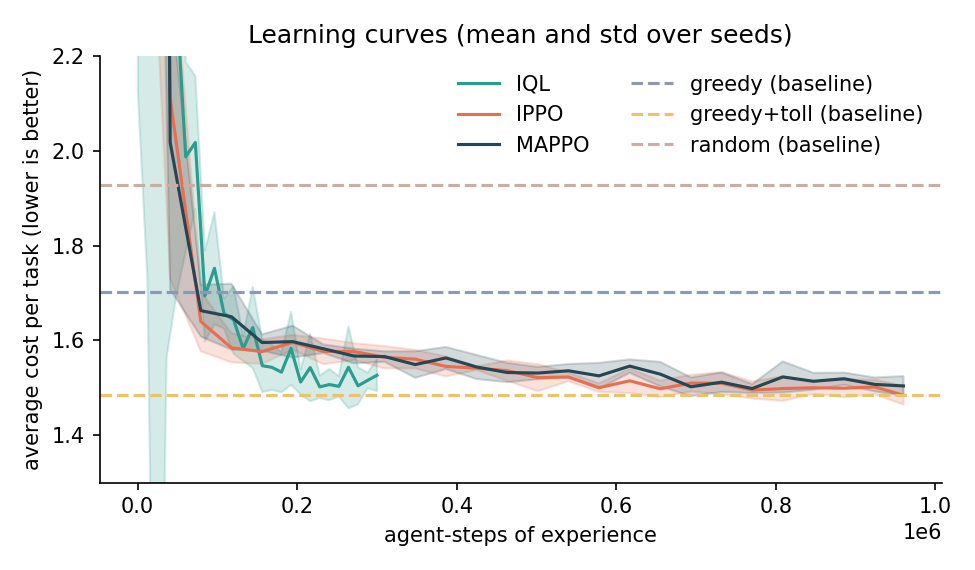
\includegraphics[width=0.78\linewidth]{learning_curves.png}
\caption{Courbes d'apprentissage (moyenne et écart-type sur 5 graines). Les lignes pointillées sont les règles de
référence.}
\label{fig:curves}
\end{figure}

Trois constats ressortent :
\begin{enumerate}
  \item \textbf{Les apprenants battent la règle myope de 10 à 12\,\%} (1,49 à 1,53 contre 1,70). Le greedy réagit
        à un signal retardé : quand le serveur paraît libre, tous les appareils s'y précipitent ensemble, la file
        déborde, puis tous repartent (effet de troupeau). Les politiques apprises utilisent l'edge un peu moins
        (45 à 49\,\% des tâches contre 54\,\%) et gardent une file plus courte (0,8 à 1,0 contre 1,5).
  \item \textbf{Les trois apprenants ne peuvent pas être départagés} : leurs intervalles de confiance se
        chevauchent. Le critique centralisé de MAPPO n'apporte pas de gain mesurable, alors même qu'il voit la
        charge réelle que les acteurs ne voient pas.
  \item \textbf{Un péage bien réglé suffit à égaler l'apprentissage} en coût moyen (1,484). L'essentiel du gain
        vient de l'internalisation de la congestion, qu'une règle à un paramètre capture déjà.
\end{enumerate}

\subsection{Asymétrie entre appareils}

\begin{figure}[h]
\centering
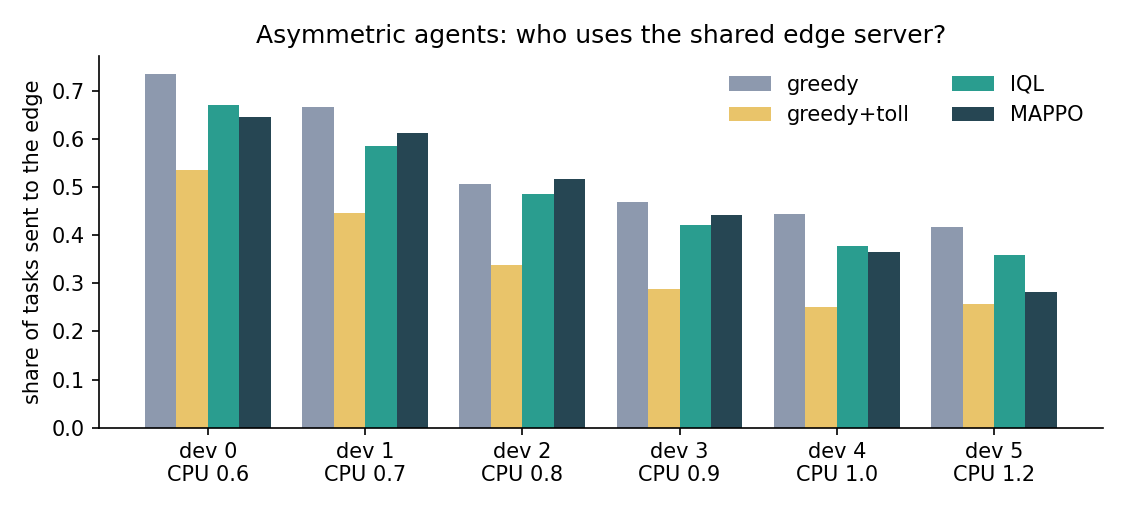
\includegraphics[width=0.8\linewidth]{per_agent_edge_share.png}
\caption{Part des tâches envoyées à l'edge par appareil (politiques apprises : moyenne sur 5 graines).}
\label{fig:agents}
\end{figure}

Toutes les politiques confient le serveur partagé surtout aux appareils lents (figure~\ref{fig:agents}). Avec
MAPPO, l'appareil le plus lent ($f=0{,}6$) y envoie 65\,\% de ses tâches et le plus rapide ($f=1{,}2$) 28\,\%.
C'est un partage efficace : un appareil rapide perd peu à calculer lui-même, alors qu'un appareil lent y perd
beaucoup. Le greedy est moins sélectif (74\,\% contre 42\,\%).

\subsection{Le prix de l'opérateur}

\begin{figure}[h]
\centering
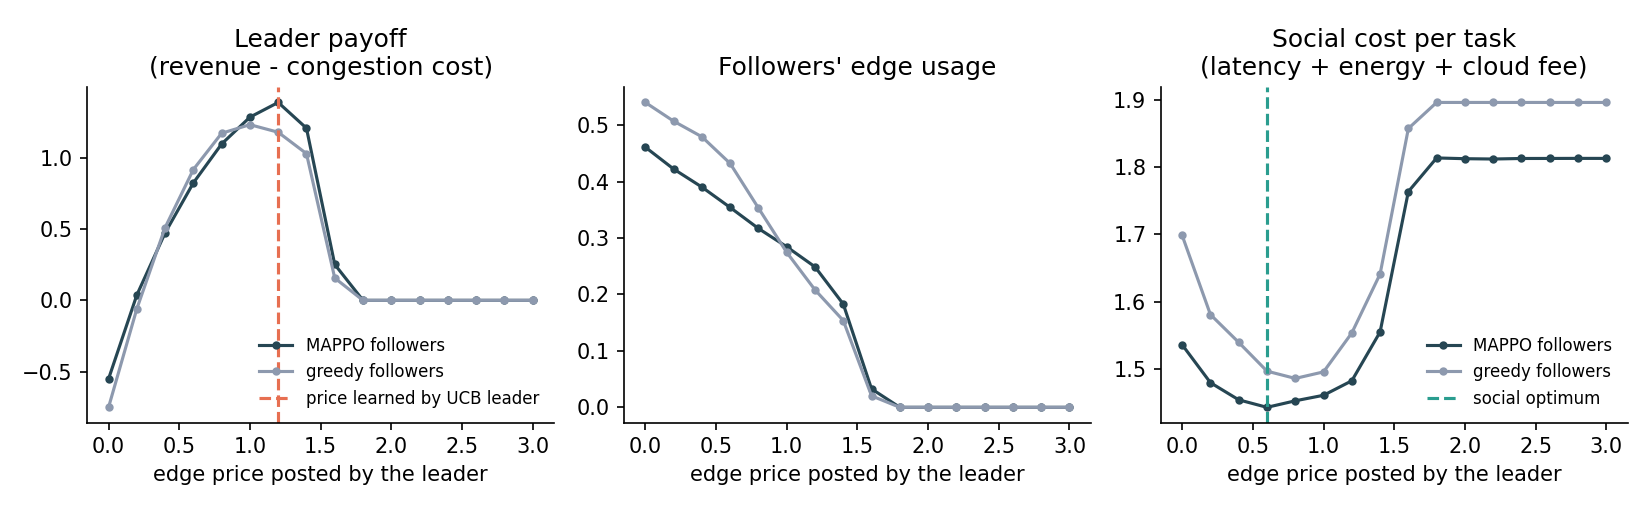
\includegraphics[width=\linewidth]{stackelberg.png}
\caption{Variante leader--suiveurs, en fonction du prix affiché : gain de l'opérateur, usage de l'edge et coût
social par tâche.}
\label{fig:stack}
\end{figure}

\begin{table}[h]
\centering\small
\begin{tabular}{ccccc}
\toprule
Prix $\pi$ & Gain de l'opérateur & Coût social / tâche & Part edge \\
\midrule
0   & $-0{,}55$ & 1,536 & 0,46 \\
0,6 & 0,82 & \textbf{1,443} & 0,35 \\
1,2 & \textbf{1,39} & 1,482 & 0,25 \\
1,6 & 0,25 & 1,764 & 0,03 \\
\bottomrule
\end{tabular}
\caption{Quelques points du balayage des prix (suiveurs MAPPO, 40 épisodes par prix).}
\end{table}

\begin{itemize}
  \item Le gain de l'opérateur est maximal pour $\pi=1{,}2$. Le bandit UCB1 retrouve ce prix, qu'il joue dans
        42\,\% des 600 épisodes.
  \item Le coût social est minimal pour $\pi=0{,}6$ : 1,443 contre 1,536 à prix nul, soit $-6$\,\%. Un prix
        modéré joue le rôle d'un péage de congestion, comme le $\theta$ de la section~3.
  \item Au-delà de $\pi\approx1{,}6$, les appareils abandonnent l'edge pour un mélange de local et de cloud.
\end{itemize}
Le prix choisi par l'opérateur est donc deux fois plus élevé que le prix socialement optimal : ses intérêts et
ceux du système ne sont pas alignés.

\subsection{Distance à l'équilibre}

\begin{table}[h]
\centering\small
\begin{tabular}{lcccc}
\toprule
Politique & NashConv & Somme brute & Gain moyen & Gains significatifs \\
\midrule
Greedy          & 0,399 & 0,378      & 3,9\,\% & 5 appareils sur 6 \\
Greedy + péage  & 0,507 & 0,507      & 5,7\,\% & 6 appareils sur 6 \\
IQL             & 0,037 & 0,035      & 0,4\,\% & 1 (appareil 4) \\
IPPO            & 0,041 & 0,040      & 0,5\,\% & 1 (appareil 5) \\
MAPPO           & 0,017 & $-0{,}011$ & 0,2\,\% & aucun \\
\bottomrule
\end{tabular}
\caption{Exploitabilité des politiques (modèles de la graine 0, 300 épisodes appariés). Un gain est significatif
si son intervalle de confiance à 95\,\% est au-dessus de zéro.}
\label{tab:nash}
\end{table}

\begin{figure}[h]
\centering
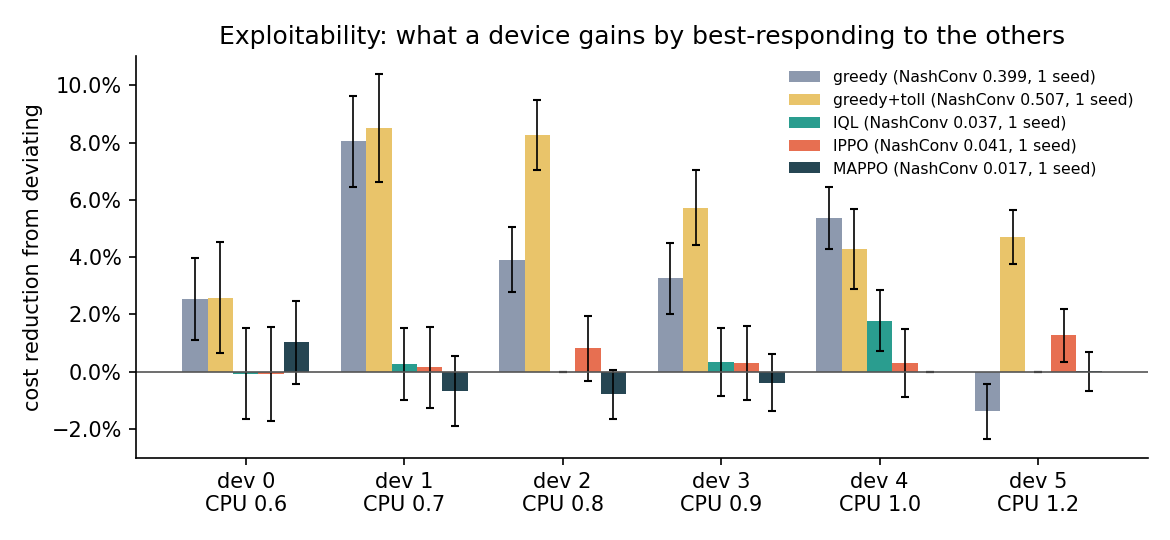
\includegraphics[width=0.8\linewidth]{exploitability.png}
\caption{Baisse de coût qu'obtient chaque appareil en déviant seul (gains bruts, IC 95\,\%).}
\end{figure}

Les politiques apprises sont bien plus proches d'un équilibre de Nash (NashConv de 0,017 à 0,041) que les deux
règles (0,399 et 0,507). Un appareil qui dévie d'une politique apprise gagne au plus 1,8\,\% de son coût, et ce
gain n'est significatif que pour deux appareils sur dix-huit. Avec la règle à péage, au contraire, chaque appareil
gagne significativement à dévier. Cette mesure nuance le constat précédent : le péage atteint le même coût moyen
que l'apprentissage, mais il n'est pas \emph{stable}, car chaque appareil aurait intérêt à ne pas le respecter.

Deux réserves. Pour les politiques apprises, la recherche est locale : sur plusieurs appareils d'IQL et de MAPPO,
l'affinage dégradait le dernier itéré et la sélection revenait à la politique de départ. Une recherche locale qui
ne trouve pas de déviation rentable est compatible avec un quasi-équilibre, sans le prouver. Pour les règles, le
meilleur point de contrôle était le dernier pour 2 (greedy) et 3 (greedy+péage) appareils sur six : ces
meilleures réponses n'ont peut-être pas convergé, et leur NashConv est une borne inférieure lâche.

%======================================================================
\section{Limites et perspectives}
%======================================================================

\paragraph{Limites.}
\begin{itemize}
  \item L'exploitabilité est une borne inférieure (meilleure réponse apprise, recherche locale pour les politiques
        apprises) et ne porte que sur une graine. L'environnement tire tout son aléa d'un seul flux : l'appariement
        par graine n'est donc pas parfait dès qu'une déviation change le nombre d'appareils sur l'edge.
  \item L'option cloud est presque toujours dominée avec ces paramètres ; le problème se réduit en pratique à
        deux actions.
  \item Le leader est statique (un prix par épisode) et les suiveurs ne s'adaptent pas à son apprentissage ; le
        bandit choisit parmi les 16 prix déjà couverts par le balayage.
  \item Le modèle reste stylisé : un seul serveur, une unité de travail abstraite, des modèles de canal et
        d'énergie simples.
\end{itemize}

\paragraph{Perspectives.}
\begin{itemize}
  \item \textbf{Réseaux de neurones sur graphes} : avec plusieurs serveurs edge et une topologie, appareils et
        serveurs forment un graphe ; un encodeur GNN permettrait de transférer une politique entre topologies et
        nombres d'agents.
  \item \textbf{Tarification dynamique apprise} : faire du leader un agent RL qui fixe le prix à chaque pas en
        fonction de la charge, entraîné conjointement avec les suiveurs (schéma à deux échelles de temps).
  \item \textbf{Objectifs coopératifs ou égoïstes} : comparer récompenses individuelles et coût social partagé, et
        mesurer le prix de l'anarchie.
  \item \textbf{Régime où le cloud compte} : réduire $D$ ou $\varphi$ pour que les trois actions soient en
        concurrence.
\end{itemize}

%======================================================================
\appendix
\section{Hyperparamètres}
%======================================================================

\begin{center}\small
\begin{tabular}{lll}
\toprule
 & Paramètre & Valeur \\
\midrule
Environnement & $N$, $H$, $p$, $F$, $d$ & 6, 50, 0,8, 3, 2 \\
              & $D$, $F_c$, $\varphi$, $\kappa$, $p_{\mathrm{tx}}$, $\lambda$ & 1,5, 10, 0,3, 0,5, 0,3, 1 \\
Réseaux       & architecture & MLP $2\times64$, $\tanh$ \\
IQL           & épisodes, mémoire, lot & 1\,000, $10^5$, 256 \\
              & pas d'apprentissage, cible, $\varepsilon$ & $5\cdot10^{-4}$, 500 pas, $1\to0{,}05$ \\
PPO           & mises à jour, épisodes / maj, passes, mini-lots & 400, 8, 4, 4 \\
              & pas d'apprentissage, $\epsilon$, $c_v$, $c_e$ & $3\cdot10^{-4}$, 0,2, 0,5, 0,01 \\
Commun        & $\gamma$, $\lambda_{\text{GAE}}$, échelle des récompenses & 0,95, 0,95, 1/3 \\
Stackelberg   & $\beta$, prix, épisodes du bandit, $c$ & 0,5, 16 dans $[0,3]$, 600, 1 \\
Exploitabilité & mises à jour (apprises / règles), épisodes d'évaluation & 150 / 300, 300 \\
\bottomrule
\end{tabular}
\end{center}

\section{Reproduire les résultats}

\begin{verbatim}
pip install -r requirements.txt
python -m pytest -q tests
python scripts/train.py --out results          # 5 graines, en parallèle
python scripts/stackelberg.py --out results
python scripts/exploitability.py --out results
python scripts/plots.py results
python scripts/report.py results               # rapport interactif HTML
\end{verbatim}

\noindent Code : \url{https://github.com/ossamasabti/marl-offload} (dépôt privé).

\end{document}
